\documentclass[11pt,a4paper]{article}
\usepackage[T1]{fontenc}
\usepackage[utf8]{inputenc}
\usepackage{lmodern}
\usepackage[french]{babel}
\usepackage{amsmath,amssymb}
\usepackage[a4paper,margin=2.2cm]{geometry}
\usepackage{booktabs}
\usepackage{float}
\usepackage{graphicx}
\usepackage{microtype}
\usepackage{enumitem}
\usepackage[hidelinks]{hyperref}

\setlist{itemsep=2pt,topsep=4pt}
\setlength{\parskip}{3pt}

% ---- Auteurs : à compléter -------------------------------------------------
\newcommand{\auteurs}{Pedro DE BEM \;\&\; Amanda FONTENELE}
% ---------------------------------------------------------------------------

\title{Projet MLSF -- Partie I\\Un solveur SAT pour la résolution du Meowdoku}
\author{\auteurs}
\date{25 octobre 2026}

% Pseudo-code numéroté léger (sans paquet externe).
\newcounter{pseudoline}
\newcounter{procedure}
\newcommand{\kw}[1]{\textbf{#1}}
\newcommand{\pinfo}[1]{\par\noindent\hspace*{2.4em}#1}
\newenvironment{pseudo}[2]
  {\par\medskip\noindent\begin{minipage}{\linewidth}\rule{\linewidth}{0.8pt}\par\noindent\refstepcounter{procedure}\label{#2}\textbf{Procédure~\theprocedure{} : #1}\par
   \noindent\rule{\linewidth}{0.4pt}\setcounter{pseudoline}{0}\small}
  {\par\noindent\rule{\linewidth}{0.8pt}\end{minipage}\par\medskip}
\newcommand{\pline}[2]{\par\stepcounter{pseudoline}\noindent
  \hbox to 1.8em{\hfil\scriptsize\thepseudoline\hspace{0.6em}}%
  \hspace*{\dimexpr 1.4em*#1\relax}%
  \parbox[t]{\dimexpr\linewidth-1.8em-1.4em*#1\relax}{#2}}
\newcommand{\occ}{\operatorname{occ}}
\newcommand{\id}{\operatorname{id}}
\newcommand{\reg}{\operatorname{reg}}

\begin{document}
\maketitle

\section*{Introduction}
Nous modélisons le jeu Meowdoku en logique propositionnelle (Question~1), implémentons l'algorithme DPLL et un lecteur DIMACS (Question~2), résolvons des grilles de bout en bout (Question~3), implémentons sept heuristiques de branchement (Question~4), les comparons sur 48 instances (Question~5) et fournissons l'interface \texttt{sat.py} demandée (Question~6). Aucune réponse fausse n'a été observée ; sur les 41 instances publiques, le mode \texttt{optimized} en résout 40 en 60\,s (\texttt{public-03} n'est résolue par aucune de nos versions). Le mode \texttt{optimized} n'est pas une implémentation plus rapide : il change seulement l'heuristique (Section~\ref{sec:q6}). Toutes les valeurs chiffrées proviennent des scripts \texttt{Q1\_script.py} à \texttt{Q6\_script.py}, dont les sorties sont dans \texttt{results/}.

\section*{Contenu du rendu et points d'attention}

\begin{table}[H]
\centering\small
\begin{tabular}{@{}p{4.3cm}p{11.3cm}@{}}
\toprule
Fichier & Rôle\\
\midrule
\texttt{meowdoku\_to\_dimacs.py} & Q1 : lecture d'une grille, encodage CNF, écriture DIMACS.\\
\texttt{generate\_grid.py} & Q1 : générateur de grilles carrées avec solution plantée.\\
\texttt{dimacs\_to\_pylist.py} & Q2 : lecteur DIMACS vers listes Python.\\
\texttt{sat.py} & Q2, Q4, Q6 : DPLL (algorithmes~1 et~2), DPLL$_H$ (algorithme~3) avec compteurs, interface en ligne de commande.\\
\texttt{heuristics.py} & Q4 : heuristiques H1, H3, H5, H7 (versions statique et dynamique).\\
\texttt{solve\_meowdoku.py} & Q3 : grille $\to$ DIMACS $\to$ DPLL $\to$ fichier solution, avec vérification.\\
\texttt{benchmark.py} & Q5, Q6 : mesures (une exécution = un processus, limite de 60\,s).\\
\texttt{Q[1-6]\_script.py} & Un script par question, qui produit les chiffres du rapport dans \texttt{results/}.\\
\texttt{make\_figures.py} & Trace la figure~\ref{fig:cactus} à partir de \texttt{results/Q5\_runs.json}.\\
\texttt{image\_grid.txt} & Grille de la figure~\ref{fig:board} au format de l'énoncé.\\
\texttt{meowdoku-instances/} & 18 formules Meowdoku (9 SAT, 9 UNSAT) et \texttt{expected.json}.\\
\texttt{public-instances/} & Instances des enseignants (41 fichiers) et \texttt{expected.json}.\\
\texttt{results/} & Sorties brutes des scripts (JSON et texte), dont les fichiers solution de la Q3.\\
\texttt{rapport/} & Sources \LaTeX{} de ce rapport.\\
\bottomrule
\end{tabular}
\caption{Fichiers du rendu. Le fichier \texttt{README.md} donne les commandes pour tout reproduire.}
\label{tab:files}
\end{table}

\paragraph{Écarts et choix par rapport à l'énoncé.}
\begin{itemize}
\item \emph{Q1} : le générateur ne traite que le cas $N=M=K$, ce que l'énoncé autorise. L'encodeur, lui, accepte $N\neq M$ et $K$ quelconque.
\item \emph{Q4} : nous implémentons H1, H3, H5 et H7 (H0 sert de référence), soit 7~configurations et H0. Nous n'avons pas implémenté H2, H4, H6, ni de heuristique propre.
\item \emph{Q5} : nous mesurons le nombre de décisions, de retours arrière, le temps CPU et la part du temps passée dans l'heuristique. Nous \emph{ne comptons pas} les propagations unitaires ni les littéraux purs (critères~3 et~4 de l'énoncé). Chaque couple (instance, heuristique) n'est exécuté \emph{qu'une fois}.
\item \emph{Q6} : le mode \texttt{optimized} utilise l'heuristique H5d avec la même propagation que le mode \texttt{dpll}. Nous n'avons pas optimisé les structures de données (voir Section~\ref{sec:q6}).
\end{itemize}

\paragraph{Éléments originaux.} Le générateur de grilles à solution plantée (Section~\ref{sec:q1}) et la construction de grilles Meowdoku \emph{insatisfiables} à partir de ce générateur (Section~\ref{sec:q5}) ne sont pas décrits dans l'énoncé. La vérification de la solution de la Q3 est indépendante du CNF. Le tracé de profils cumulés (figure~\ref{fig:cactus}) est emprunté à la pratique des compétitions SAT.

% TODO : ajouter ici le paragraphe \paragraph{Usage des assistants IA.} (exigé par l'énoncé).

\paragraph{Conventions.} Les variables sont numérotées comme en DIMACS ; un littéral $l$ vaut $p$ ou $\neg p$, et $\bar l$ désigne le littéral opposé. Toutes les mesures ont été faites sur la machine de l'annexe~\ref{sec:setup}, qui n'est \emph{pas} celle de la compétition ; les temps absolus ne sont donc pas comparables à ceux de la compétition.

% =============================================================================
\section{Question 1 : modélisation et génération de grilles}\label{sec:q1}

\subsection{Variables et clauses}

Pour une grille de $N$ lignes, $M$ colonnes et $K$ régions $R_1,\dots,R_K$, on introduit une variable $x_{i,j}$ par case, vraie si et seulement si la case $(i,j)$ contient un chat. Elle est numérotée $\id(i,j)=(i-1)M+j$, de $1$ à $NM$. La figure~\ref{fig:board} sert d'exemple fil rouge ($N=M=K=6$). Les clauses sont les suivantes.
\begin{align*}
F_{\text{lignes}}&=\bigwedge_{i,\;j<k}(\neg x_{i,j}\lor\neg x_{i,k}) &&\text{au plus un chat par ligne},\\
F_{\text{colonnes}}&=\bigwedge_{j,\;i<k}(\neg x_{i,j}\lor\neg x_{k,j}) &&\text{au plus un chat par colonne},\\
F_{\text{régions}}&=\bigwedge_{r=1}^{K}\Bigl[\bigl(\textstyle\bigvee_{u\in R_r}x_u\bigr)\land\bigwedge_{\{u,v\}\subseteq R_r,\,u\ne v}(\neg x_u\lor\neg x_v)\Bigr] &&\text{exactement un chat par région},\\
F_{\text{diag.}}&=\bigwedge_{i<N,\;j<M}(\neg x_{i,j}\lor\neg x_{i+1,j+1})\land(\neg x_{i,j+1}\lor\neg x_{i+1,j}) &&\text{pas de chats diagonaux}.
\end{align*}
Le voisinage à huit cases est couvert sans clause supplémentaire : deux cases voisines horizontalement ou verticalement sont dans la même ligne ou la même colonne, donc déjà exclues par $F_{\text{lignes}}$ et $F_{\text{colonnes}}$ ; les voisines en diagonale sont les deux diagonales d'un bloc $2\times2$, traitées par $F_{\text{diag.}}$.

\begin{figure}[H]
\centering
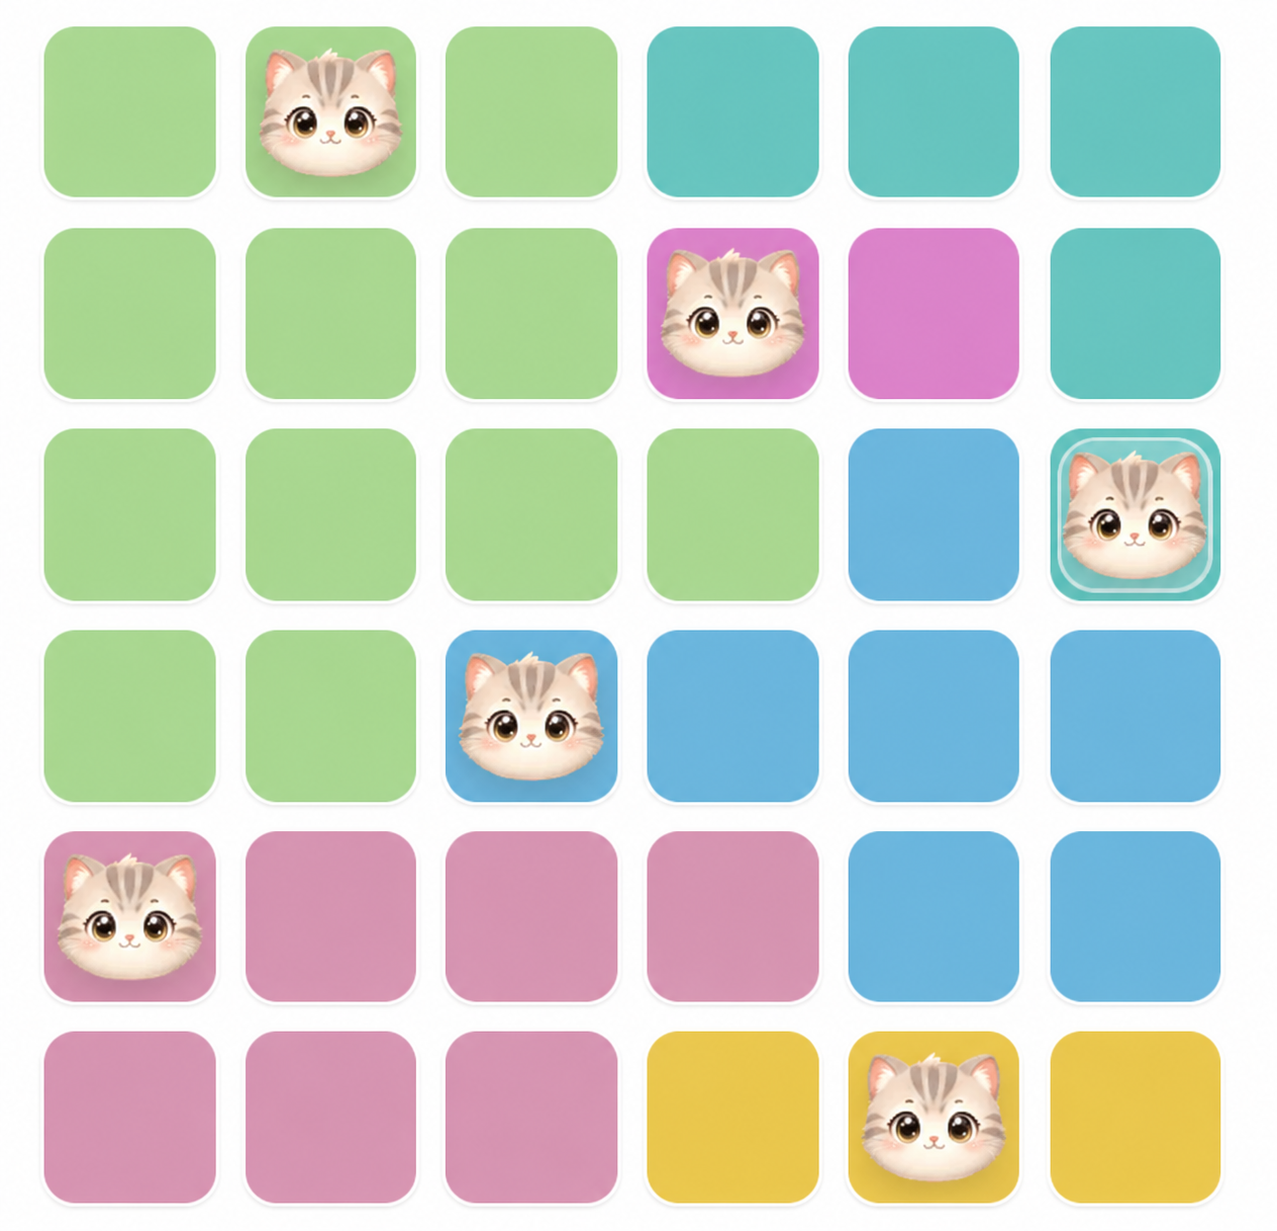
\includegraphics[width=0.36\linewidth]{figures/meowdoku_board.png}
\caption{Grille $6\times6$ utilisée comme exemple ; les chats montrent l'unique solution.}
\label{fig:board}
\end{figure}

\paragraph{Correction de l'encodage.} Une valuation satisfaisant $F=F_{\text{lignes}}\land F_{\text{colonnes}}\land F_{\text{régions}}\land F_{\text{diag.}}$ place les chats sur les variables vraies ; chaque ligne et colonne en contient au plus un, chaque région exactement un, et deux chats ne se touchent pas. Réciproquement, tout placement légal définit une valuation qui satisfait chaque clause. Il y a donc une bijection entre les placements légaux et les modèles de $F$ (les variables sont uniquement les cases, aucune variable auxiliaire). Sur la grille de la figure~\ref{fig:board}, nous avons testé les $6!=720$ placements à un chat par ligne et colonne : un seul satisfait les 358 clauses, celui de la figure.

\paragraph{Taille (analyse de complexité).} Le nombre de variables est $NM$. Le nombre de clauses est $N\binom M2+M\binom N2+\sum_{r}\bigl(1+\binom{s_r}2\bigr)+2(N-1)(M-1)$, où $s_r=|R_r|$ : il est quadratique en la taille des lignes, colonnes et régions, soit $O(NM^2+MN^2+\sum_r s_r^2)$. Pour la figure~\ref{fig:board}, on obtient $90+90+128+50=358$ clauses (tailles des régions $12,5,2,7,7,3$) ; pour une grille générée $50\times50$, 196\,650 clauses. Nous n'éliminons pas les doublons (par exemple $\{\neg x_2,\neg x_3\}$ est émise par la règle des lignes et par celle de la région A) ; ils sont sans effet sur la satisfiabilité.

Le convertisseur \texttt{meowdoku\_to\_dimacs.py} lit le format de la figure~1b de l'énoncé (lignes \texttt{c} ignorées, \texttt{GRID}, \texttt{ZONES}, puis $N$ lignes d'étiquettes), vérifie la cohérence (noms distincts, nombre de lignes et de colonnes, étiquettes utilisées exactement celles déclarées), puis écrit le fichier DIMACS dont l'en-tête est \texttt{p cnf} $NM$ $|F|$.

\subsection{Génération de grilles satisfiables}

Le générateur (\texttt{generate\_grid.py}, cas $N=M=K=n$) \emph{plante} d'abord une solution, puis dessine les régions autour : la grille est satisfiable par construction.
\begin{enumerate}[label=\textbf{\arabic*.}]
\item \emph{Placement des chats.} On cherche, par retour arrière avec ordre aléatoire, des colonnes $c_1,\dots,c_n$ deux à deux distinctes avec $|c_i-c_{i+1}|\ge2$. Il y a donc un chat par ligne et par colonne, et deux chats de lignes consécutives ne se touchent pas (ceux de lignes plus éloignées non plus). Pour $n\ge4$, une solution existe toujours (colonnes paires croissantes puis impaires croissantes) ; pour $n=2$ et $3$, il n'y en a pas, et le générateur le signale.
\item \emph{Croissance des régions.} La région $R_i$ est amorcée par le chat de la ligne $i$. Un parcours en largeur multi-sources (file FIFO, voisins en ordre aléatoire) étend chaque région aux cases voisines encore sans région. Chaque case reçoit exactement une région, la région $R_i$ contient son seul chat, et elle est connexe. La grille est donc valide et le placement planté en est une solution.
\end{enumerate}
La graine du générateur aléatoire rend les grilles reproductibles. Le générateur garantit \emph{au moins} une solution, pas l'unicité (la grille $5\times5$ de graine~1 en a 7), et ne tire pas uniformément parmi les grilles valides : le parcours en largeur produit des régions compactes de tailles inégales (de 14 à 93 cases pour $n=50$). Le générateur produit une grille $50\times50$ en 4\,ms ; l'essentiel du coût est celui de l'encodage ensuite.

% =============================================================================
\section{Question 2 : lecture de DIMACS et algorithme DPLL}\label{sec:q2}

\subsection{Représentation et lecture}

Une formule est une liste de clauses, une clause est une liste d'entiers non nuls (convention DIMACS). La formule sans clause est \texttt{[]} (satisfiable) et celle qui contient la clause vide est par exemple \texttt{[[1, 2], [], [-1]]} (insatisfiable) ; le lecteur distingue bien les deux cas, présents dans les instances \texttt{edge\_no\_clause\_sat} et \texttt{edge\_empty\_clause\_unsat}. Le lecteur (\texttt{read\_dimacs}) accepte les clauses sur plusieurs lignes, ignore les commentaires, et rejette avec un message explicite : en-tête absent ou mal formé, littéral hors de $1..V$, dernière clause sans \texttt{0}, nombre de clauses différent de celui annoncé. Son coût est linéaire en la taille du fichier.

\subsection{DPLL : une procédure pour les trois algorithmes}

Les algorithmes~1 (statut), 2 (statut et valuation) et 3 (heuristique $H$) de l'énoncé ne diffèrent que par le retour de la fonction et le choix de la ligne~17. Nous les implémentons par une seule procédure (\texttt{dpll\_h} dans \texttt{sat.py}) ; \texttt{dpll\_status} et \texttt{dpll\_model} sont les algorithmes~1 et~2 avec le choix aléatoire $H_0$.

\begin{pseudo}{DPLL$_H$($F$) : statut et valuation}{proc:dpll}
\pline{0}{\kw{si} $F$ contient une clause vide \kw{alors retourner} (UNSAT, $\emptyset$)}
\pline{0}{\kw{si} $F$ ne contient aucune clause \kw{alors retourner} (SAT, $\emptyset$)}
\pline{0}{\kw{si} $F$ contient une clause unitaire $\{l\}$, ou à défaut un littéral pur $l$, \kw{alors}}
\pline{1}{$(s,v)\leftarrow$ DPLL$_H$(Simplifier($F,l$))}
\pline{1}{\kw{si} $s=$ SAT \kw{alors retourner} (SAT, $v\cup\{l\}$) \kw{sinon retourner} (UNSAT, $\emptyset$)}
\pline{0}{$l\leftarrow H(F)$ \hfill (littéral choisi : $l=p$ signifie $p\leftarrow1$, $l=\neg p$ signifie $p\leftarrow0$)}
\pline{0}{\kw{pour} $l'$ dans $(l,\bar l)$}
\pline{1}{$(s,v)\leftarrow$ DPLL$_H$(Simplifier($F,l'$))}
\pline{1}{\kw{si} $s=$ SAT \kw{alors retourner} (SAT, $v\cup\{l'\}$)}
\pline{0}{\kw{retourner} (UNSAT, $\emptyset$)}
\end{pseudo}
Simplifier($F,l$) est la formule $F[l\leftarrow1]$ : on retire les clauses contenant $l$ et on retire $\bar l$ des autres. Choix d'implémentation :
\begin{itemize}
\item La valuation est un dictionnaire variable $\to$ booléen, construit au retour de la récursion ; UNSAT est représenté par \texttt{None}. Les variables sans valeur peuvent prendre n'importe quelle valeur ; l'interface leur donne la valeur fausse.
\item La clause unitaire utilisée est la première de la liste ; à défaut, le littéral pur de plus petit numéro de variable. \texttt{simplify} construit une nouvelle liste, ce qui rend le retour arrière trivial (la formule d'origine est intacte) mais coûte une copie à chaque affectation.
\item Chaque appel affecte au moins une variable : la profondeur peut atteindre le nombre de variables. Nous relevons la limite de récursion de Python et exécutons la recherche dans un thread à pile de 256\,Mio (\texttt{run\_deep}). Sans cela, \texttt{public-06} (1363 variables) échoue par \texttt{RecursionError}.
\end{itemize}

\paragraph{Complexité.} Chaque nœud de l'arbre coûte $O(|F|)$ : test de clause vide, recherche d'une clause unitaire, collecte des littéraux pour le littéral pur, et copie par \texttt{simplify}. La profondeur est au plus le nombre $n$ de variables et chaque décision a deux branches, donc le pire cas est $O(2^n\cdot|F|)$ : la complexité est exponentielle, comme l'énoncé le rappelle. En pratique, la taille de l'arbre dépend fortement de l'ordre de branchement (Q4--Q5).

\subsection{Validation et performances}

\paragraph{Protocole.} Les 41 fichiers des enseignants sont lus, puis chacun est résolu \emph{trois fois} par chaque version (\texttt{dpll\_status} et \texttt{dpll\_model}, via \texttt{sat.py}), avec 60\,s par exécution ; trois fois parce que le choix de branche est aléatoire. Le statut est comparé à \texttt{expected.json} et chaque modèle est vérifié contre toutes les clauses. Les temps sont des médianes, mesurées avec huit exécutions en parallèle, donc indicatives.

\paragraph{Résultats.} Sur 246 exécutions, aucune réponse n'est fausse. Trente-sept instances sont résolues à chaque exécution par les deux versions ; \texttt{public-03} et \texttt{public-27} ne sont jamais résolues, \texttt{public-06} et \texttt{public-12} seulement parfois. Les 19 autres instances de benchmark ont une médiane d'au plus 0{,}5\,s. La table~\ref{tab:q2} donne les instances lentes.
\begin{table}[H]
\centering\small
\begin{tabular}{@{}lrrcll@{}}
\toprule
Instance & Variables & Clauses & Statut & \texttt{dpll\_model} & \texttt{dpll\_status}\\
\midrule
\texttt{public-03} & 63 & 168 & UNSAT & 0/3, timeout & 0/3, timeout\\
\texttt{public-06} & 1363 & 3034 & SAT & 0/3, timeout & 1/3, 0,5 s\\
\texttt{public-08} & 100 & 900 & UNSAT & 3/3, 1,8 s & 3/3, 0,7 s\\
\texttt{public-11} & 729 & 21844 & SAT & 3/3, 36,8 s & 3/3, 13,5 s\\
\texttt{public-12} & 522 & 11636 & SAT & 1/3, 7,1 s & 1/3, 3,3 s\\
\texttt{public-15} & 100 & 850 & UNSAT & 3/3, 1,9 s & 3/3, 2,6 s\\
\texttt{public-18} & 459 & 7054 & SAT & 3/3, 21,0 s & 3/3, 10,7 s\\
\texttt{public-19} & 729 & 22060 & SAT & 3/3, 2,1 s & 3/3, 3,3 s\\
\texttt{public-22} & 100 & 850 & UNSAT & 3/3, 3,0 s & 3/3, 3,0 s\\
\texttt{public-27} & 181 & 3151 & SAT & 0/3, timeout & 0/3, timeout\\
\texttt{public-30} & 100 & 850 & UNSAT & 3/3, 3,5 s & 3/3, 1,5 s\\
\bottomrule
\end{tabular}
\caption{Instances dont la médiane dépasse 1\,s ou qui ne sont pas toujours résolues. « $k$/3, $t$ » : $k$ exécutions sur 3 terminées en 60\,s, $t$ médiane de leurs temps.}
\label{tab:q2}
\end{table}

\paragraph{Commentaires.}
\begin{itemize}
\item \emph{Temps instable.} Avec le choix aléatoire, \texttt{public-12} est résolue en 3,3\,s dans une exécution de \texttt{dpll\_status} et dépasse 60\,s dans les deux autres ; \texttt{public-18} varie de 10,1 à 56,8\,s. Les écarts entre \texttt{dpll\_status} et \texttt{dpll\_model} (par exemple 11\,s contre 21\,s sur \texttt{public-18}) sont du même ordre : les deux versions font la même recherche et nos mesures ne montrent pas que l'une soit plus rapide.
\item \emph{\texttt{public-03}} est insatisfiable avec seulement 63 variables mais aucune de nos six exécutions ne la résout en 60\,s : l'arbre complet doit être parcouru. Le README des enseignants prévient que certaines instances sont difficiles pour un DPLL de base.
\item \emph{Coût du pas.} La copie de la formule à chaque affectation pèse sur les grosses instances : \texttt{public-11} et \texttt{public-19} (environ 22\,000 clauses) prennent de 2 à 37\,s.
\end{itemize}

% =============================================================================
\section{Question 3 : résolution d'une grille Meowdoku}\label{sec:q3}

Le programme \texttt{solve\_meowdoku.py} prend un fichier grille et écrit un fichier solution. Il enchaîne les briques précédentes (Procédure~\ref{proc:solve}).
\begin{pseudo}{Résolution d'un fichier grille}{proc:solve}
\pline{0}{lire la grille ($N$, $M$, noms de régions, $\reg(i,j)$) ; $F\leftarrow$ clauses de la grille (Q1)}
\pline{0}{écrire $F$ dans un fichier DIMACS temporaire, puis le relire avec le lecteur de la Q2}
\pline{0}{$(s,v)\leftarrow$ DPLL($F$) ; \kw{si} $s=$ UNSAT \kw{alors} signaler « pas de solution » (code retour 1, aucun fichier écrit)}
\pline{0}{$P\leftarrow\{(\lfloor (t-1)/M\rfloor+1,\;((t-1)\bmod M)+1)\mid t\text{ vraie dans }v\}$}
\pline{0}{vérifier $P$ avec Vérifier (ci-dessous) ; \kw{si} une violation est détectée \kw{alors} l'afficher et s'arrêter}
\pline{0}{écrire : copie du fichier grille ; une ligne « \texttt{région ligne colonne} » par région, dans l'ordre de \texttt{ZONES} ; la grille où \texttt{*} marque un chat et \texttt{.} une case vide}
\end{pseudo}
La recherche passe bien par un fichier DIMACS, comme demandé ; le fichier temporaire est supprimé ensuite. La ligne~4 inverse $\id(i,j)=(i-1)M+j$ : sur la figure~\ref{fig:board}, la variable 35 donne la case $(6,5)$.

\paragraph{Vérification indépendante.} La fonction \texttt{check\_solution} n'utilise que la grille et les positions des chats, jamais le CNF : pour chaque région le nombre de chats doit être 1, et pour chaque paire de chats les lignes et colonnes doivent différer et $\max(|i-i'|,|j-j'|)\ge2$. Elle détecte donc une erreur d'encodage, de traduction ou de solveur.

\paragraph{Tests.} (Sorties dans \texttt{results/Q3\_results.txt}.)
\begin{itemize}
\item Sur la grille de la figure~1b de l'énoncé, le fichier écrit contient exactement la solution de sa figure~2 (\texttt{A 3 2}, \texttt{B 2 5}, \texttt{C 1 3}, \texttt{D 5 6}, \texttt{E 4 4}, \texttt{F 6 1}).
\item Sur la grille de la figure~\ref{fig:board}, dont la solution est unique, le programme retrouve les chats en $(1,2),(2,4),(3,6),(4,3),(5,1),(6,5)$.
\item Des placements illégaux (deux chats sur une ligne, deux chats en diagonale, un chat déplacé dans une colonne occupée) sont tous signalés ; le placement légal ne l'est pas.
\item Une grille $2\times2$ (régions \texttt{A A} / \texttt{B B}) est déclarée sans solution.
\item Des grilles générées (graines 1, 2, 3, $n$ de 4 à 20) sont toutes résolues et validées (table~\ref{tab:q3}).
\end{itemize}
\begin{table}[H]
\centering\small
\begin{tabular}{@{}rrccc@{}}
\toprule
$n$ & Variables & Graine 1 & Graine 2 & Graine 3\\
\midrule
4 & 16 & 0,07 s & 0,07 s & 0,07 s\\
8 & 64 & 0,09 s & 0,08 s & 0,08 s\\
12 & 144 & 0,14 s & 0,10 s & 0,08 s\\
15 & 225 & 0,16 s & 1,21 s & 5,07 s\\
20 & 400 & 2,58 s & 0,41 s & 7,00 s\\
\bottomrule
\end{tabular}
\caption{Temps de résolution de grilles générées $n\times n$ (une exécution, DPLL à choix aléatoire, démarrage de l'interpréteur compris ; $n=6,10$ omis).}
\label{tab:q3}
\end{table}
Jusqu'à $n=12$, une grille se résout en environ 0,1\,s ; pour $n=15$ et $20$, le temps dépend de la grille et des choix aléatoires (de 0,16 à 7\,s).

% =============================================================================
\section{Question 4 : heuristiques de branchement}\label{sec:q4}

\subsection{Heuristiques implémentées}

La fonction $H$ de la procédure~\ref{proc:dpll} choisit un littéral : on essaie $l\leftarrow1$ d'abord. Avec $\occ_k(l,F)$ le nombre d'occurrences de $l$ dans les clauses de taille $k$ de $F$, $\occ(l,F)=\sum_k\occ_k(l,F)$ et $k_{\min}$ la taille de la plus petite clause :
\begin{table}[H]
\centering\small
\begin{tabular}{@{}llp{5.2cm}l@{}}
\toprule
Heuristique & Score d'un littéral $l$ & Idée & Versions\\
\midrule
H1 (PVL) & aucun : plus petite variable de $F$, valeur 1 & coût nul, référence & H1\\
H3 (LP) & $\occ(l,F)$ & littéral le plus fréquent & H3s, H3d\\
H5 (LFCM) & $\occ_{k_{\min}}(l,F)$ & le plus fréquent dans les clauses les plus courtes & H5s, H5d\\
H7 (LJW) & $\sum_k\occ_k(l,F)\,2^{-k}$ & Jeroslow--Wang : les clauses courtes pèsent plus & H7s, H7d\\
\bottomrule
\end{tabular}
\caption{Heuristiques implémentées. $H_0$ (choix aléatoire) sert de référence.}
\label{tab:heur}
\end{table}
Le littéral de score maximal est choisi ; l'égalité est départagée par le plus petit numéro de variable, puis par le littéral positif. La version \emph{dynamique} recalcule les scores sur la formule courante à chaque décision. La version \emph{statique} les calcule une fois sur la formule initiale, classe les littéraux, puis renvoie à chaque décision le premier littéral classé dont la variable apparaît encore dans $F$. Cela donne les huit configurations $H_0$, H1, H3s, H3d, H5s, H5d, H7s, H7d.

\paragraph{Respect des contraintes de l'énoncé.} Heuristique fondée sur un littéral : H3, H5, H7 (H1 et H$_0$ choisissent la variable). Heuristique utilisant les tailles de clauses : H5, H7. Heuristique dynamique : H3d, H5d, H7d.

\paragraph{Raisons des choix.} H3 est l'heuristique de littéral la plus simple. Une clause courte devient unitaire en premier, et la propagation unitaire est le moyen le moins cher de couper la recherche ; H5 ne regarde que les clauses les plus courtes, et H7 pondère toutes les clauses par $2^{-k}$, ce qui favorise les courtes sans ignorer les autres. H1 ne coûte rien à calculer et montre ce qu'une heuristique calculée doit apporter. Proposer les versions statique et dynamique de H3, H5 et H7 permet de mesurer en Q5 ce que rapporte le recalcul et ce qu'il coûte.

\paragraph{Coût.} Une décision dynamique est en $O(|F|)$ (parcours de $F$ pour compter les littéraux). La version statique coûte $O(|F_0|\log|F_0|)$ une fois, mais notre implémentation parcourt aussi $F$ à chaque décision (pour savoir quelles variables restent) : son coût est donc aussi en $O(|F|)$, avec une constante plus faible.

\subsection{Validation}
Les huit configurations donnent la bonne réponse, et un modèle valide en cas de SAT, sur les 11 petites instances des enseignants (interface, cas limites : 88 exécutions, aucune fausse, \texttt{results/Q4\_validation.txt}), ainsi que sur les 30 instances de benchmark et les 18 formules Meowdoku de la Q5 (les instances non résolues en 60\,s ne donnent pas de réponse).

% =============================================================================
\section{Question 5 : comparaison des heuristiques}\label{sec:q5}

\subsection{Protocole}

\paragraph{Instances.} Les 30 instances de benchmark des enseignants (19 SAT, 11 UNSAT) et 18 formules Meowdoku. Neuf sont satisfiables : grilles de taille $n=10,15,20$, graines 1, 2, 3, du générateur de la Q1. Neuf sont insatisfiables : $n=8,9,10$, mêmes graines, construites ainsi (Procédure~\ref{proc:unsat}).
\begin{pseudo}{Grille Meowdoku insatisfiable de taille $n$ et de graine $s$}{proc:unsat}
\pline{0}{générer la grille de taille $n$ et de graine $s$, avec ses chats plantés}
\pline{0}{$E\leftarrow$ cases sans chat, dans l'ordre de lecture ; affecter à ses trois premières cases une nouvelle région $X$}
\pline{0}{\kw{retourner} la grille, qui a $n+1$ régions pour $n$ lignes}
\end{pseudo}
Il faut un chat par région, soit $n+1$ chats, mais au plus un par ligne : la formule est insatisfiable. Nous donnons trois cases à la région $X$ et non une, car une région d'une seule case donne une clause unitaire et la propagation unitaire réfute alors la formule sans aucune recherche.

\paragraph{Mesures.} Chaque couple (instance, heuristique) est exécuté une fois, dans un processus propre, limité à 60\,s, dix processus à la fois. $H_0$ est aléatoire : son résultat est donc un seul échantillon. Critères : nombre de \emph{décisions} (exécutions de la ligne~17 de l'algorithme~3), temps CPU, part du temps CPU passée dans l'heuristique. Le nombre de \emph{retours arrière} (exécutions de la branche \texttt{else}) vaut de 97,9\,\% à 99,5\,\% du nombre de décisions pour toutes les heuristiques (sur les instances résolues par toutes), donc il n'apporte presque rien en plus et n'est pas détaillé. Les compteurs ne modifient pas la recherche. Aucune des 384 exécutions n'a donné de réponse fausse (statut comparé à l'attendu, modèle vérifié sur toutes les clauses).

\subsection{Résultats}

\begin{table}[H]
\centering\small
\begin{tabular}{@{}lrrrrr@{}}
\toprule
 & Publiques SAT & Publiques UNSAT & Meowdoku SAT & Meowdoku UNSAT & Total\\
 & (19) & (11) & (9) & (9) & (48)\\
\midrule
$H_0$ & 17 & 10 & 9 & 9 & 45\\
H1 & 18 & 10 & 8 & 9 & 45\\
H3s & 18 & 10 & 7 & 9 & 44\\
H3d & 18 & 10 & 9 & 9 & 46\\
H5s & 18 & 10 & 8 & 9 & 45\\
H5d & 19 & 10 & 9 & 9 & \textbf{47}\\
H7s & 17 & 10 & 7 & 9 & 43\\
H7d & 17 & 10 & 9 & 9 & 45\\
\bottomrule
\end{tabular}
\caption{Instances résolues en 60\,s (effectif entre parenthèses).}
\label{tab:solved}
\end{table}
La table~\ref{tab:solved} compte les instances résolues. \texttt{public-03} n'est résolue par aucune heuristique. Les autres échecs : \texttt{public-12} ($H_0$, H1, H3s, H5s, H7s), \texttt{public-06} ($H_0$, H7s, H7d), \texttt{public-11} (H3d, H7d), \texttt{sat-n20-s1} (H3s, H5s, H7s) et \texttt{sat-n20-s2} (H1, H3s, H7s).

L'effort est comparé sur les instances résolues par \emph{toutes} les heuristiques (16 publiques SAT, 10 publiques UNSAT, 7 Meowdoku SAT, 9 Meowdoku UNSAT) : table~\ref{tab:effort}.
\begin{table}[H]
\centering\footnotesize
\setlength{\tabcolsep}{4pt}
\begin{tabular}{@{}lrrrrrrrrr@{}}
\toprule
 & \multicolumn{2}{c}{Publiques SAT} & \multicolumn{2}{c}{Publiques UNSAT} & \multicolumn{2}{c}{Meowdoku SAT} & \multicolumn{2}{c}{Meowdoku UNSAT} & Part\\
 & Déc. & CPU & Déc. & CPU & Déc. & CPU & Déc. & CPU & heur.\\
\midrule
$H_0$ & 13,1\,k & 70,0 s & 9,4\,k & 15,3 s & 3,1\,k & 2,1 s & 24,1\,k & 15,3 s & 1,8\,\%\\
H1 & 6,9\,k & 66,4 s & 5,2\,k & 7,2 s & 39,1\,k & 29,0 s & 1,4\,k & 1,5 s & 2,0\,\%\\
H3s & 24,1\,k & 31,9 s & 3,4\,k & 5,0 s & 33,2\,k & 19,4 s & 33,0\,k & 15,5 s & 3,3\,\%\\
H3d & 28,0\,k & 50,9 s & 2,3\,k & 3,4 s & 2,4\,k & 3,4 s & 48,4\,k & 17,2 s & 8,7\,\%\\
H5s & 6,8\,k & 37,0 s & 1,2\,k & 0,5 s & 33,2\,k & 17,6 s & 33,0\,k & 18,5 s & 2,9\,\%\\
H5d & 57,9\,k & 77,3 s & 1,0\,k & 0,5 s & 2,4\,k & 3,5 s & 48,4\,k & 18,8 s & 10,8\,\%\\
H7s & 5,3\,k & 29,0 s & 1,2\,k & 0,6 s & 33,2\,k & 16,4 s & 33,0\,k & 15,2 s & 3,0\,\%\\
H7d & 18,4\,k & 62,7 s & 1,0\,k & 0,5 s & 2,4\,k & 3,8 s & 48,4\,k & 18,4 s & 9,7\,\%\\
\bottomrule
\end{tabular}
\caption{Total des décisions (milliers) et du temps CPU par groupe, sur les instances résolues par toutes les heuristiques, et part du temps CPU passée dans l'heuristique (sur les quatre groupes).}
\label{tab:effort}
\end{table}

\begin{figure}[H]
\centering
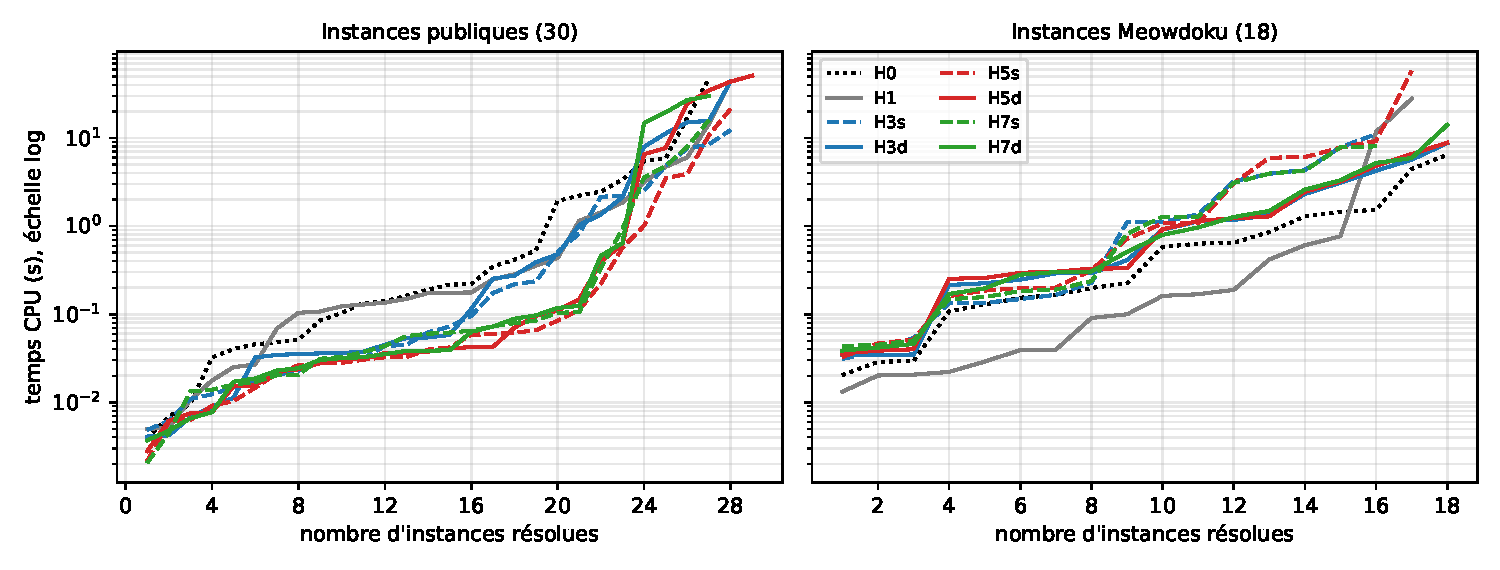
\includegraphics[width=\linewidth]{figures/cactus.pdf}
\caption{Profils cumulés : pour chaque heuristique, temps CPU des instances résolues, triés par ordre croissant (échelle logarithmique). Plus une courbe est basse et longue, mieux c'est.}
\label{fig:cactus}
\end{figure}

\subsection{Analyse}

\paragraph{Les résultats sont-ils conformes à nos attentes ?} En partie. Nous attendions que les heuristiques battent le choix aléatoire, que le dynamique batte le statique et que les heuristiques à tailles de clauses battent les simples.
\begin{itemize}
\item \emph{Heuristique contre aléatoire.} Vrai sur les instances publiques UNSAT : H5 et H7 font environ 1\,000 décisions contre 9\,400 pour $H_0$, et 0,5 à 0,6\,s de CPU contre 15,3\,s. Faux sur Meowdoku : en SAT, $H_0$ résout les sept grilles en 2,1\,s, plus vite que toutes les autres ; en UNSAT, les heuristiques à fréquence font plus de décisions que $H_0$ (33\,000 à 48\,400 contre 24\,100), seule H1 fait mieux (1\,400).
\item \emph{Dynamique contre statique.} Vrai sur Meowdoku SAT (2\,400 décisions contre 33\,200). Faux sur les publiques SAT (H5d : 57\,900 décisions, H5s : 6\,800) et sur Meowdoku UNSAT (48\,400 contre 33\,000).
\item \emph{Tailles de clauses.} Sur les publiques UNSAT, H5 et H7 sont bien meilleures que H1 et H3 ; sur les publiques SAT, H7s est la plus rapide (29,0\,s), mais H3d est plus rapide que H5d et H7d.
\end{itemize}
Sur les grilles Meowdoku, les trois versions dynamiques prennent \emph{exactement} les mêmes décisions (mêmes totaux). Nous supposons que c'est dû à la structure de la formule : presque toutes les clauses sont binaires et négatives (au plus un chat), donc les trois scores désignent le même littéral. Nous n'avons pas vérifié cette explication. Sur Meowdoku UNSAT, H1 est la meilleure : nous supposons que brancher dans l'ordre des cases épuise rapidement les premières lignes et révèle le manque de chats, sans avoir vérifié non plus.

\paragraph{Dans quelle mesure une heuristique améliore-t-elle DPLL (algorithme 2) ?} Cela dépend de la famille. Sur les publiques UNSAT, H5 et H7 divisent le temps CPU par 25 à 30. Sur les publiques SAT, H7s prend 29,0\,s contre 70,0\,s pour $H_0$. Sur Meowdoku, il n'y a pas de gain avec nos heuristiques à fréquence (sauf H1 en UNSAT). Le nombre d'instances résolues augmente peu : 47 pour H5d contre 45 pour $H_0$, qui échoue sur \texttt{public-06} et \texttt{public-12} ; comme $H_0$ est un seul tirage, ces écarts sont indicatifs.

\paragraph{Le recalcul dynamique est-il rentable ?} Le calcul de l'heuristique représente de 9 à 11\,\% du temps CPU en dynamique contre environ 3\,\% en statique. Le recalcul rapporte sur Meowdoku SAT : de 4 à 6 fois plus rapide (3,4 à 3,8\,s contre 16,4 à 19,4\,s) et les neuf grilles sont résolues, ce qu'aucune version statique ne fait. Il rapporte aussi sur \texttt{public-12}, que ni $H_0$ ni les versions statiques ne résolvent. Il ne rapporte pas sur les publiques SAT (H3d, H5d et H7d sont plus lentes que leurs versions statiques : 50,9, 77,3 et 62,7\,s contre 31,9, 37,0 et 29,0\,s) ni sur les UNSAT (temps comparables). Aucune heuristique n'est la meilleure partout ; selon le nombre d'instances résolues, premier critère du classement, H5d est la meilleure.

\paragraph{Limites de l'étude.} Une seule exécution par couple ; $H_0$ n'est qu'un échantillon ; les totaux ne portent que sur les instances résolues par toutes les heuristiques, ce qui exclut les instances difficiles et sous-estime les heuristiques qui résolvent plus d'instances ; dix processus tournent en parallèle, ce qui perturbe les temps ; les propagations unitaires et littéraux purs ne sont pas comptés.

% =============================================================================
\section{Question 6 : interface et mode optimisé}\label{sec:q6}

\paragraph{Interface.} La commande est \texttt{python sat.py instance.cnf}, avec les options \texttt{-{}-mode dpll}, \texttt{-{}-mode optimized} et \texttt{-{}-output-model}. Le mode par défaut est \texttt{dpll}. La sortie standard contient \texttt{s SATISFIABLE} ou \texttt{s UNSATISFIABLE} et, avec \texttt{-{}-output-model} pour une formule satisfiable, une ligne \texttt{v} listant les variables de 1 à $V$ avec leur signe et terminée par \texttt{0} (variable sans valeur : fausse) ; aucun modèle pour une formule insatisfiable. Rien d'autre n'est écrit sur la sortie standard, les erreurs vont sur la sortie d'erreur. Les deux modes partagent le même format et donnent le même statut.

\paragraph{Mode \texttt{optimized}.} C'est DPLL$_H$ avec l'heuristique H5d. Nous l'avons choisie d'après la Q5, parce qu'elle résout le plus d'instances (47 sur 48) et que le nombre d'instances résolues est le premier critère de classement. Elle est déterministe, donc reproductible. \emph{La propagation et les structures de données sont celles du mode \texttt{dpll}} : ce n'est pas une implémentation plus rapide, seulement un autre ordre de branchement.

\paragraph{Vérification.} Les deux modes ont été exécutés par la ligne de commande sur les 41 instances publiques, une fois chacun, 60\,s, huit à la fois. Une réponse est correcte si le statut est le bon et, pour SAT, si le modèle satisfait toutes les clauses.
\begin{table}[H]
\centering\small
\begin{tabular}{@{}lrr@{}}
\toprule
Mode & Réponses correctes (sur 41) & Temps total de ces réponses\\
\midrule
\texttt{dpll} & 39 & 51,8 s\\
\texttt{optimized} & 40 & 134,7 s\\
\bottomrule
\end{tabular}
\caption{Les deux modes sur les 41 instances publiques.}
\label{tab:q6}
\end{table}
Aucune réponse n'est fausse. Le mode \texttt{dpll} ne résout ni \texttt{public-03} ni \texttt{public-27}. Le mode \texttt{optimized} résout \texttt{public-27} (40,7\,s) mais pas \texttt{public-03}. Sur les 39 instances résolues par les deux, il est plus lent (94,0\,s contre 51,8\,s), surtout sur \texttt{public-06} (35,1\,s contre 0,6\,s) et \texttt{public-12} (25,9\,s contre 12,4\,s), que le mode \texttt{dpll} a résolues vite grâce à des choix aléatoires favorables (cf.~Q2).

\paragraph{Limites et pistes.} Le gain d'une instance (\texttt{public-27}) se fait avec une marge faible : 40,7\,s et 35,1\,s sur \texttt{public-06} pour une limite de 60\,s, sur une machine différente de celle de la compétition. Le goulot d'étranglement est la propagation : la copie de $F$ à chaque affectation et le parcours complet pour trouver les clauses unitaires. Les pistes les plus directes sont une propagation unitaire par compteurs ou \emph{watched literals} avec un historique d'affectations défaisable (plus de copie), des index littéral $\to$ clauses, et une boucle itérative. Nous ne les avons pas réalisées.

% =============================================================================
\section{Bilan}\label{sec:bilan}

L'encodage est vérifié de façon exhaustive sur la grille exemple et, indépendamment, par \texttt{check\_solution} ; le solveur est correct sur toutes les instances disponibles (aucune réponse fausse sur les 41 instances publiques et les 18 formules Meowdoku). Ses faiblesses sont la vitesse (une instance publique non résolue, plusieurs résolues près de la limite) et le protocole de mesure (une exécution par couple, critères partiels), signalées ci-dessus. Le point le plus utile pour la suite serait de remplacer la propagation par copie par une propagation incrémentale.

\appendix
\section{Environnement expérimental}\label{sec:setup}

\begin{table}[H]
\centering\small
\begin{tabular}{@{}p{4.2cm}p{11.2cm}@{}}
\toprule
Machine & Acer Nitro ANV16-42-R3JW\\
Processeur & AMD Ryzen 7 260, x86\_64, 8 c\oe urs physiques, 16 CPU logiques\\
Mémoire & 14 Gio de RAM (DDR5, 5600\,MT/s), 4 Gio de swap\\
Système & Ubuntu 26.04.1 LTS, noyau Linux 7.0.0-38-generic\\
Python & CPython 3.14.4 (la compétition utilise Python 3.12 ; la syntaxe du code a été vérifiée pour 3.12, mais il n'a pas été exécuté sous 3.12)\\
Parallélisme & Q2 : 8 processus à la fois ; Q5 : 10 ; Q6 : 8 ; Q3 : un seul\\
\bottomrule
\end{tabular}
\caption{Configuration utilisée pour toutes les mesures. Elle diffère de celle de la compétition (Core Ultra 7 155H, Ubuntu 22.04, Python 3.12, Docker limité à 4 CPU et 8\,Gio).}
\end{table}

\section{Reproduction}
Depuis la racine du rendu, avec Python $\ge3.12$ (la figure demande \texttt{matplotlib}) :
\begin{verbatim}
python3 sat.py public-instances/instances/smoke_01_sat.cnf \
        --mode optimized --output-model
python3 meowdoku_to_dimacs.py image_grid.txt grid.cnf
python3 generate_grid.py 8 grille8.txt --seed 1
python3 solve_meowdoku.py image_grid.txt solution.txt
python3 Q1_script.py     # ... jusqu'à Q6_script.py ; écrit dans results/
python3 make_figures.py                           # rapport/figures/cactus.pdf
\end{verbatim}
Les scripts Q2, Q5 et Q6 lancent des centaines d'exécutions limitées à 60\,s et peuvent durer longtemps.

\end{document}
